% \chapter{Ứng dụng phân tích mã nguồn Rust bằng đồ thị CPG}
\chapter{Ứng dụng thực nghiệm và đánh giá}
\label{chap:experiment}

% Chương 5 trình bày về cách ánh xạ cây AST sang đồ thị CPG trên các thể loại cú pháp Rust.
% Mức độ cài đặt và các hạn chế hiện thời của công cụ sẽ được thảo luận.
% Không chỉ vậy, công cụ sẽ được sử dụng để phân tích mã nguồn của một số đoạn mã có lỗ hổng bảo mật được công bố trên RUSTSEC Database \cite{rustsecAboutRustSec}.
% Ngoài ra, chương cũng sẽ thực nghiệm ứng dụng đồ thị CPG trong bài toán học máy phân loại mã nguồn Rust có lỗ hổng bảo mật, thực hiện so sánh với mô hình học máy khác và chứng minh tiềm năng khai thác của đồ thị CPG dành cho ngôn ngữ Rust.

Chương 4 trình bày về các ứng dụng phân tích mã nguồn Rust bằng đồ thị CPG bao gồm phân tích mã nguồn có lỗ hổng và kĩ thuật học máy.
Công cụ được sử dụng để phân tích mã nguồn của một số đoạn mã có lỗ hổng bảo mật được công bố trên RUSTSEC Database \cite{rustsecAboutRustSec}.
Chương cũng sẽ thực nghiệm ứng dụng đồ thị CPG trong bài toán học máy phân loại mã nguồn Rust có lỗ hổng bảo mật, thực hiện so sánh với mô hình học máy khác và chứng minh tiềm năng khai thác của đồ thị CPG dành cho ngôn ngữ Rust.

% \section{Cài đặt công cụ}

Theo thư viện \href{https://docs.rs/syn/2.0.87/syn/}{syn v2.0.87}, phiên bản hiện thời có định nghĩa của 162 \texttt{struct} tương ứng với 162 loại nút AST và 33 \texttt{enum} tương ứng với 33 loại nút AST đa hình.
Hiện tại công cụ đã ánh xạ 162 loại nút AST và 33 loại nút AST đa hình ở trên thành một loại nút CPG tương ứng, tức là 100\% định nghĩa các loại nút AST đã được ánh xạ sang nút CPG.
Bảng tổng hợp ánh xạ 1-1 từ nút AST sang nút CPG tương ứng được trình bày tại địa chỉ \href{TODO}{TODO}.

Công cụ được thực hiện kiểm thử trên 151 tệp mã nguồn bao gồm đa dạng các thể loại cú pháp, thu thập từ trang \href{https://doc.rust-lang.org/stable/rust-by-example/index.html}{Rust By Example} thuộc Rust Foundation \cite{rustlangRustFoundation}.
Ngoài ra, việc chuyển đổi từ AST sang CPG được kiểm tra trên 20 dự án lớn nằm trong 100 dự án Rust có lượng sao lớn nhất trên Github \cite {githubGithubRankingTop100RustmdMaster}.
Mã nguồn của công cụ được lưu trữ tại địa chỉ \href{https://github.com/congnghiahieu/rust-parser}{rust-parser}, \href{https://github.com/congnghiahieu/syn-serde}{syn-serde}, \href{https://github.com/congnghiahieu/joern}{joern}, \href{https://github.com/congnghiahieu/codepropertygraph}{codepropertygraph}.

% \section{Các cú pháp đã hỗ trợ}

Phần này sẽ trình bày một số cú pháp của Rust khác biệt so với ngôn ngữ C/C++ và cách mà công cụ đã hỗ trợ cho các cú pháp này.
Các cú pháp bao gồm: if let, while let, match, lifetime.
Những đoạn mã nguồn và hình ảnh mô tả đồ thị CPG được sử dụng từ giờ đến cuối chương đã được đơn giản hóa để dễ dàng thể hiện và minh họa.
Các cạnh và các nút không phải trọng tâm của đồ thị CPG đã được loại bỏ để tập trung vào các tính năng cần trình bày.

\subsection{Cú pháp if let}
If else là cấu trúc điều khiển có mặt trong tất cả các loại ngôn ngữ phổ biến.
Nó cho phép chúng ta kiểm tra một điều kiện và thực thi một khối mã nếu điều kiện đúng và một khối mã khác nếu điều kiện sai.
Cấu trúc câu lệnh if else sẽ bao gồm một điều kiện và 2 khối mã.
Nếu điều kiện đúng, khối mã trong if sẽ được thực thi, ngược lại khối mã trong else sẽ được thực thi.
Thông thường khối điều kiện sẽ là biểu thức trả về kết quả đúng hoặc sai của biểu thức đó.
Trong ngôn ngữ như C/C++ thì chỉ chấp nhận biểu thức điều kiện, việc sử dụng mệnh đề có dấu hai chấm để kết thúc câu lệnh là không hợp lệ.

Với phương châm \texttt{"Expression over statement"} và nhằm mục đích tạo sự ngắn gọn, Rust cho phép thực hiện phép khai báo biến và gán giá trị cho biến trong cùng một câu lệnh bằng điều kiện if let.
Cú pháp của câu lệnh if let như sau:

\begin{minted}[mathescape, breaklines, frame=lines, framesep=2mm, baselinestretch=1.2, fontsize=\footnotesize, linenos]{rust}
if let <pattern> = <expression> {
     <block>
} else {
     <block>
}
\end{minted}

\usemintedstyle{default}

Cú pháp này sẽ thực hiện 2 công việc, kiểm tra xem \texttt{<expression>} có khớp với \texttt{<pattern>} hay không, nếu không khớp thì trả về $false$, nếu có khớp thì tiếp tục thực hiện tạo biến mới dựa theo \texttt{<pattern>} vừa lấy được và trả về $true$.
Các biến được khai báo mới từ \texttt{<pattern>} sẽ có phạm vi tồn tại trong khối lệnh điều kiện thành công.
Do thực hiện 2 công việc trong cùng 1 câu lệnh nên khi quy đổi sang câu lệnh tương tự trong ngôn ngữ như C/C++ sẽ tương đương 2 câu lệnh kiểm tra điều kiện và gán biến.

\begin{listing}[H]
\begin{minted}[mathescape, breaklines, frame=lines, framesep=2mm, baselinestretch=1.2, fontsize=\footnotesize, linenos]{rust}
let number: Option<i32> = None;
let i_like_letters = false;

if let Some(i) = number {
    println!("Matched number {:?}!", i);
} else if i_like_letters {
    // ...
} else {
    // ...
}
\end{minted}
\caption{Ví dụ mã nguồn cho if let}
\label{code:c5_iflet}
\end{listing}

\begin{listing}[H]
\begin{minted}[mathescape, breaklines, frame=lines, framesep=2mm, baselinestretch=1.2, fontsize=\footnotesize, linenos]{cpp}
Object* obj = inputObj();

if (obj != nullptr) { // 1 câu lệnh kiểm tra điều kiện
    int number = *static_cast<int*>(obj); // 1 câu lệnh gán biến
    std::cout << "Matched " << number << "!" << std::endl;
}
\end{minted}
\caption{Ví dụ mã nguồn cho if let tương đương trong C++}
\label{code:c5_iflet_cpp}
\end{listing}

Trong hình \ref{img:c5_cpg_iflet}, cạnh \texttt{CONDITION} của nút \texttt{ExprIf} trỏ tới nút \texttt{Assignment}, đồng thời cũng khai báo biến mới với tên $i$.
Các mệnh đề trong khối được thực thi khi điều kiện đúng nếu có nhắc tới biến $i$ thì sẽ tham chiếu tới biến $i$ vừa được khai báo thông qua cạnh \texttt{REF}.

\begin{figure}[H]
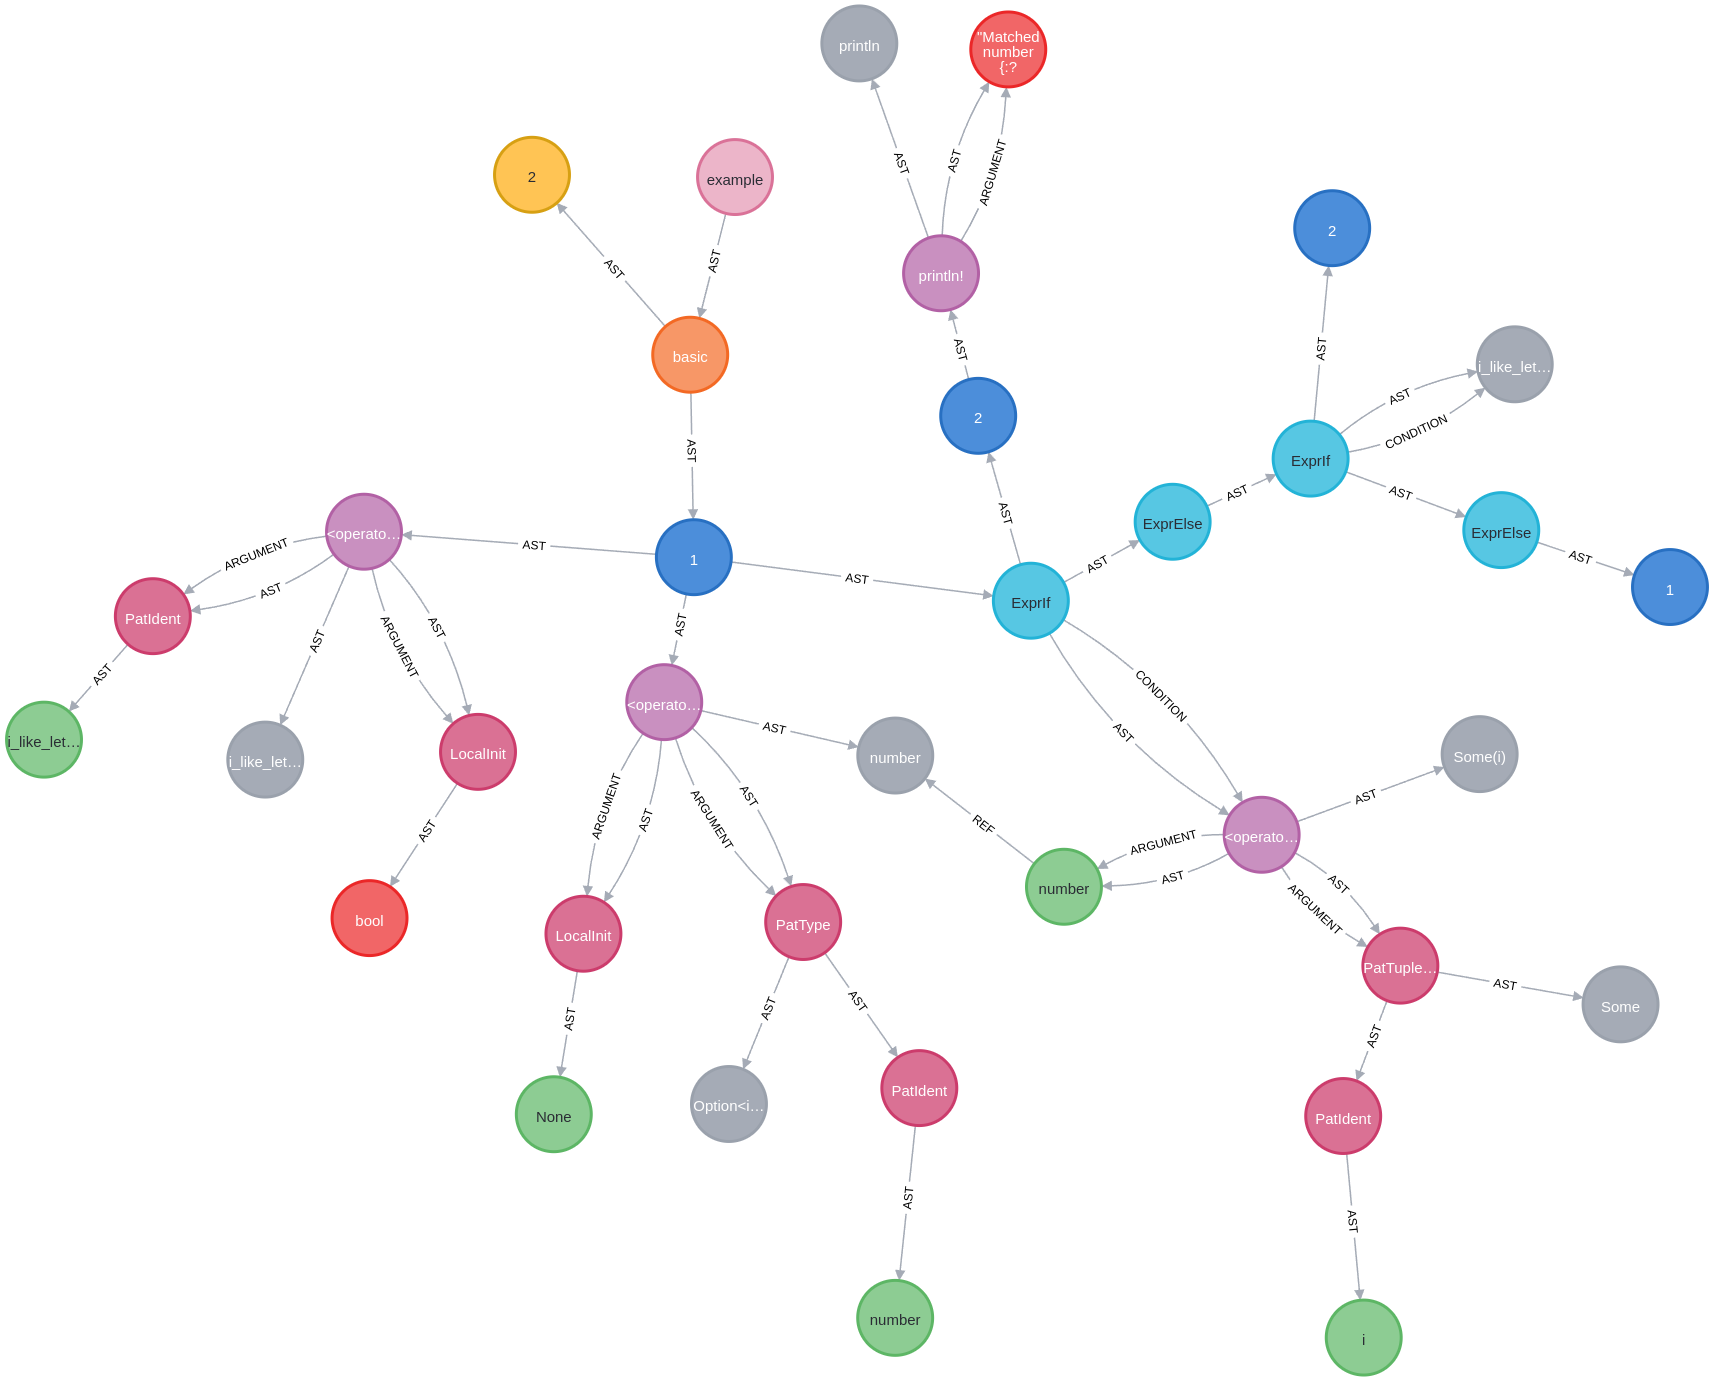
\includegraphics[width=1\columnwidth]{figures/c5/c5_iflet.png}
\centering
\caption{Ví dụ đồ thị CPG cho đoạn mã nguồn if let \ref{code:c5_iflet}}
\label{img:c5_cpg_iflet}
\end{figure}

\subsection{Cú pháp while let}

Tương tự với tính năng if let ở trên, Rust cũng hỗ trợ việc khai báo biến làm điều kiện cho vòng lặp while. Cú pháp của vòng lặp while let như sau:

\begin{minted}[mathescape, breaklines, frame=lines, framesep=2mm, baselinestretch=1.2, fontsize=\footnotesize, linenos]{rust}
while let <pattern> = <expression> {
        <block>
}
\end{minted}

Có thể hiểu là nếu việc khớp giữa \texttt{<pattern>} và \texttt{<expression>} thành công thì sẽ tiếp tục thực hiện vòng lặp, sẽ có 1 biến $i$ mới được khởi tạo đối với mỗi lần lặp.
Các mệnh đề trong khối được thực thi điều kiện của vòng lặp thành công sẽ tham chiếu tới biến $i$ vừa được khai báo thông qua cạnh \texttt{REF} nếu có sử dụng tới.
Không chỉ vậy vế phải của điều kiện \texttt{<expression>} có thể được gán lại liên tục trong quá trình lặp, nếu \texttt{<pattern>} không khớp kết thúc vòng lặp.

\begin{listing}[H]
\begin{minted}[mathescape, breaklines, frame=lines, framesep=2mm, baselinestretch=1.2, fontsize=\footnotesize, linenos]{rust}
let mut optional = Some(0);

while let Some(i) = optional {
    if i > 9 {
        optional = None;
    } else {
        optional = Some(i + 1);
    }
}
\end{minted}
\caption{Ví dụ mã nguồn cho while let}
\label{code:c5_whilelet}
\end{listing}

\begin{figure}[H]
    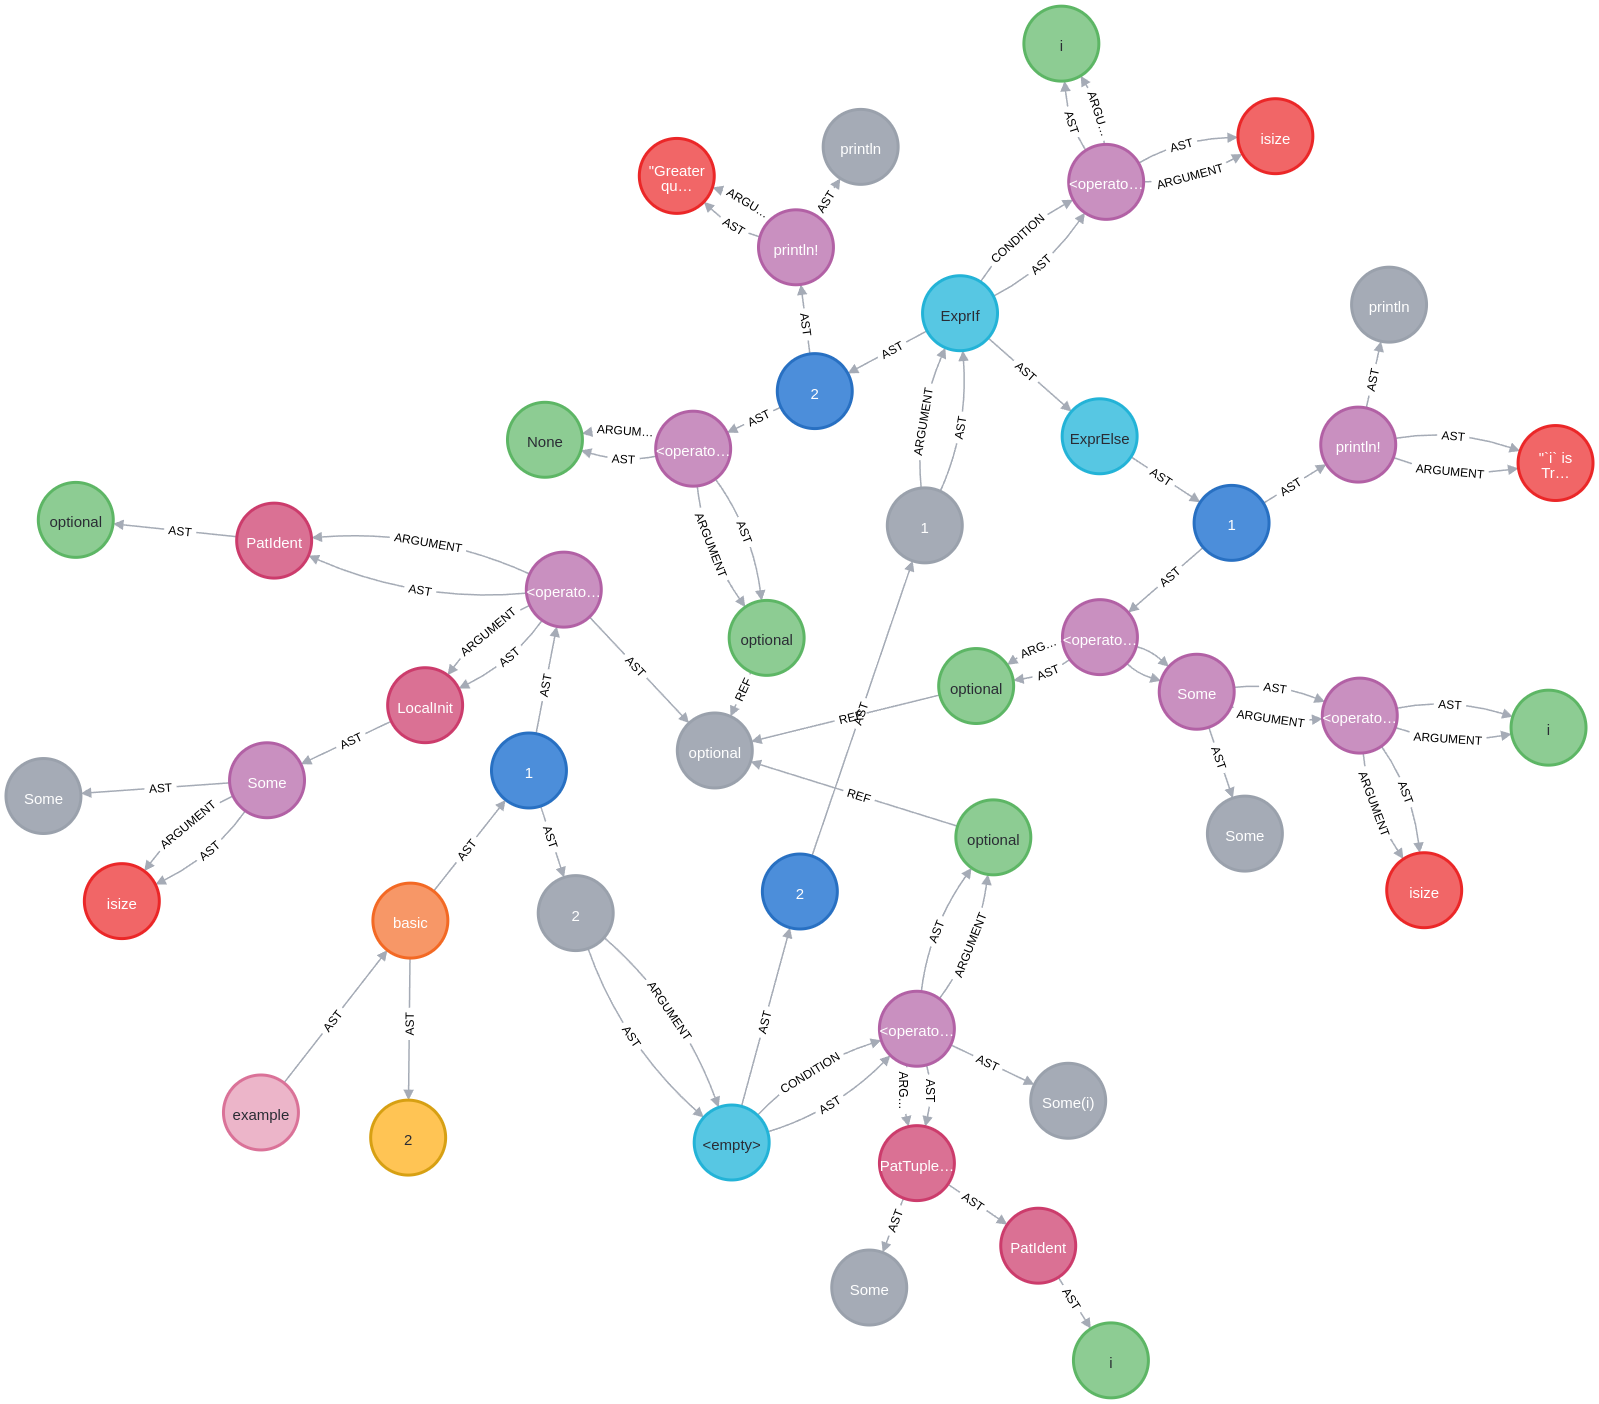
\includegraphics[width=1\columnwidth]{figures/c5/c5_whilelet.png}
    \centering
    \caption{Ví dụ đồ thị CPG cho đoạn mã nguồn while let \ref{code:c5_whilelet}}
    \label{img:c5_cpg_whilelet}
\end{figure}

\subsection{Cú pháp match}

Ngoài việc sử dụng mệnh đề gán biến thành biểu thức điều kiện, tính hướng hàm của Rust còn thể hiện ở tính năng match với sự kết hợp giữa Pattern matching và Algebraic Data Types.
Cấu trúc match không chỉ kiểm tra giá trị mà còn kết hợp với các pattern phức tạp, bao gồm kiểm tra điều kiện, kiểm tra các kiểu dữ liệu khác nhau và so sánh.
Điều này mang lại cho Rust tính linh hoạt cao hơn so với switch trong C/C++ khi chỉ so sánh giá trị nguyên thủy.

Một điểm khác biệt quan trọng giữa match và switch là tính toàn diện của match.
Rust yêu cầu các pattern trong match phải bao quát tất cả các khả năng có thể xảy ra, nếu không trình biên dịch sẽ báo lỗi.
Điều này giúp đảm bảo rằng không có tình huống nào bị bỏ qua, tăng cường độ an toàn của mã nguồn.
Trong khi đó, switch trong C/C++ không yêu cầu bao quát tất cả các trường hợp, và việc bỏ sót một trường hợp có thể dẫn đến lỗi hoặc hành vi không mong muốn.
Thêm vào đó, match trong Rust cho phép trích xuất và xử lý các thành phần của cấu trúc dữ liệu phức tạp ngay trong quá trình đối chiếu pattern.
Ví dụ, Rust có thể match trên \texttt{tuple}, \texttt{enum}, \texttt{struct}, trong khi switch của C/C++ thường chỉ giới hạn trong các giá trị nguyên thủy.

\begin{listing}[H]
\begin{minted}[mathescape, breaklines, frame=lines, framesep=2mm, baselinestretch=1.2, fontsize=\footnotesize, linenos]{rust}
enum Color {
    Red,
    Blue(u32, u32, u32),
    Green { red: u32, green: u32, blue: u32, },
}

fn main() {
    let color = Color::Blue(0, 0, 255);

    match color {
        Color::Red => println!("The color is Red!")
        Color::Blue(r, g, b) => println!("R: {}, G: {}, B: {}!", r, g, b)
        Color::Green {red, green, blue} => println!("R: {}, G: {}, B: {}!", red, green, blue),
    }
}
\end{minted}
\caption{Ví dụ mã nguồn cho match}
\label{code:c5_match}
\end{listing}

\begin{figure}[H]
    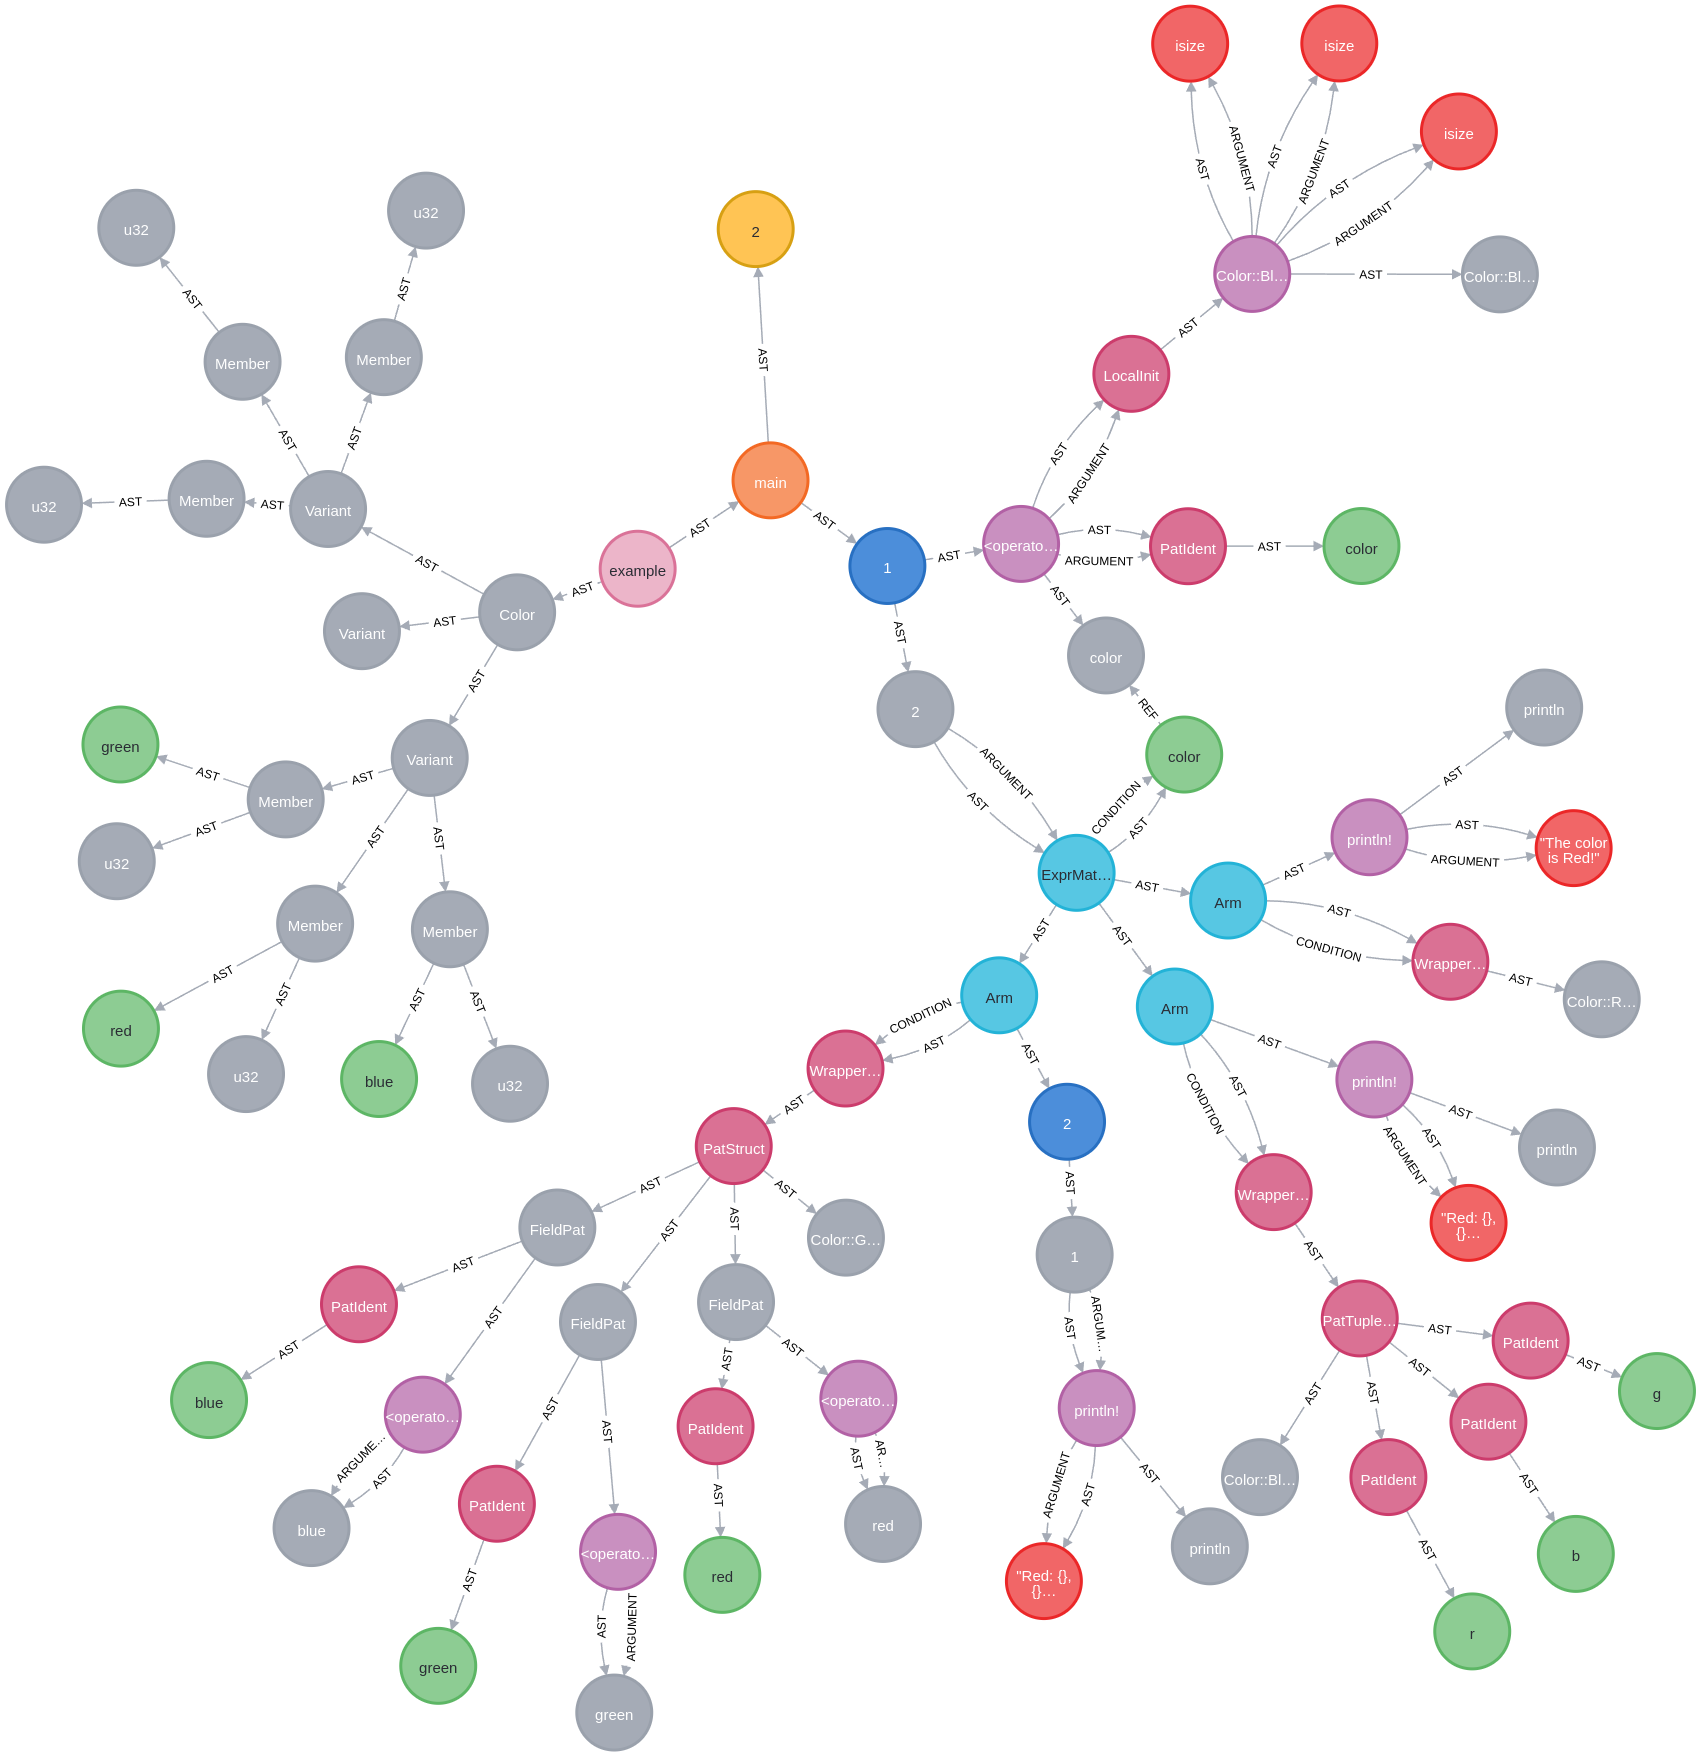
\includegraphics[width=1\columnwidth]{figures/c5/c5_match.png}
    \centering
    \caption{Ví dụ đồ thị CPG cho đoạn mã nguồn match \ref{code:c5_match}}
    \label{img:c5_match}
\end{figure}

\subsection{Cú pháp lifetime}

Lifetime là cơ chế được sử dụng trong Rust để quản lý vòng đời của các biến tham chiếu, đảm bảo rằng các biến tham chiếu không trỏ tới vùng nhớ không còn tồn tại.
Lifetime có vai trò tương tự như kiểu tổng quát, nhưng thay vì định kiểu cho biến thì lifetime sẽ xác định vòng đời cho biến tham chiếu.
Để biểu diễn được tính năng lifetime trên đồ thị CPG, có 3 loại nút mới được thêm vào đặc tả CPG là \texttt{Lifetime}, \texttt{LifetimeParameter}, \texttt{LifetimeArgument}.
Ngoài ra còn có cạnh \texttt{OUT\_LIVE} được bổ sung để chỉ ra quan hệ giữa biến và lifetime, quan hệ giữa các lifetime với nhau.

\texttt{LifetimeParameter} và \texttt{LifetimeArgument} được sử dụng cho các \texttt{struct}, \texttt{enum}, \texttt{trait} để chỉ ra lifetime tổng quát cho các biến tham chiếu.
Loại nút \texttt{Lifetime} sẽ thể hiện vòng đời thực sự của biến tham chiếu.
Các biến tham chiếu sẽ được gán lifetime thông qua việc sử dụng dấu "\texttt{'}" trước tên lifetime, ví dụ như \texttt{'a}.
Nếu các biến cùng đánh dấu lifetime \texttt{'a} thì sẽ có cạnh \texttt{OUT\_LIVE} trỏ từ biến tới nút \texttt{Lifetime} đại diện cho \texttt{'a} tương ứng.
Nếu lifetime \texttt{'a} được giới hạn bởi lifetime \texttt{'b} thì sẽ có cạnh \texttt{OUT\_LIVE} từ nút \texttt{Lifetime} \texttt{'a} tới nút \texttt{Lifetime} \texttt{'b}.

Ownership, borrowing và lifetime là 3 tính năng làm nên cơ chế an toàn bộ nhớ trong Rust.
Do vậy đồ thị CPG phải thể hiện được 3 tính năng trên đồ thị và cung cấp thông tin thông qua các nút, cạnh và thuộc tính phù hợp.
Đặc biệt là tính năng lifetime, vòng đời hợp lệ của các biến được thể hiện qua lifetime do đó việc thể hiện đúng quan hệ giữa lifetime và biến, lifetime với lifetime, biến với biến là rất quan trọng.
Từ đó có thể khai thác thông tin để kiểm tra vòng đời của biến tham chiếu, giúp phát hiện được các lỗi về bộ nhớ gây ra khi đánh dấu lifetime không chính xác.

% Lifetime elision là cơ chế trong Rust giúp tự động suy diễn lifetime cho các biến tham chiếu.
% Có ba luật chính về lifetime elision trong Rust.
% Thứ nhất, mỗi biến tham chiếu đầu vào sẽ được tự động gán lifetime mà không cần phải đánh dấu một cách tường minh.
% Thứ hai, nếu hàm có chỉ có một biến tham chiếu đầu và một biến tham chiếu đầu ra, trình biên dịch sẽ suy luận rằng biến tham chiếu đầu ra có cùng lifetime với biến tham chiếu đầu vào.
% Cuối cùng, nếu hàm có một hoặc nhiều hơn một biến tham chiếu đầu vào và một trong biến đầu vào là biến \texttt{self} (\texttt{self} tương đương với \texttt{this} trong C/C++), trình biên dịch sẽ suy luận rằng biến tham chiếu đầu ra có cùng lifetime với \texttt{self}.
% Ngoài 3 trường hợp trên, Rust yêu cầu phải ghi rõ lifetime cho tất cả các biến tham chiếu để tránh nhầm lẫn và đảm bảo an toàn bộ nhớ.

\begin{listing}[H]
\begin{minted}[mathescape, breaklines, frame=lines, framesep=2mm, baselinestretch=1.2, fontsize=\footnotesize, linenos]{rust}
fn longest<'a>(x: &'a str, y: &'a str) -> &'a str {
    if x.len() > y.len() {
        x
    } else {
        y
    }
}
\end{minted}
\caption{Ví dụ mã nguồn cho lifetime cho hàm}
\label{code:c5_lifetime_1}
\end{listing}

\begin{figure}[H]
    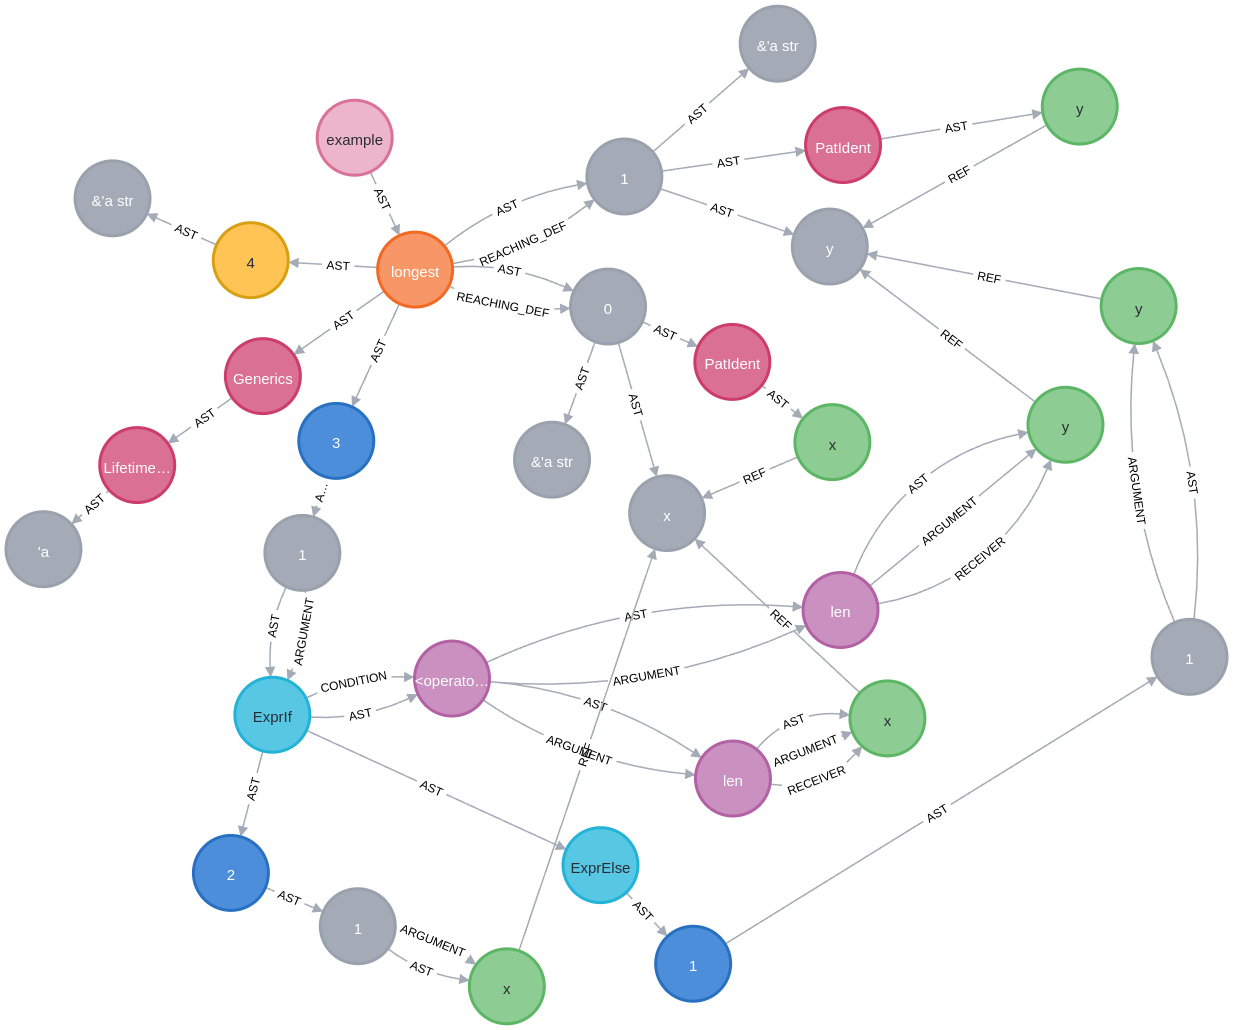
\includegraphics[width=1\columnwidth]{figures/c5/c5_lifetime_1.png}
    \centering
    \caption{Ví dụ đồ thị CPG cho đoạn mã nguồn \ref{code:c5_lifetime_1}}
    \label{img:c5_lifetime_1}
\end{figure}

\begin{listing}[H]
\begin{minted}[mathescape, breaklines, frame=lines, framesep=2mm, baselinestretch=1.2, fontsize=\footnotesize, linenos]{rust}
fn f<'a, 'b, 'c, 'd: 'c>(x: &'a i32, mut y: &'b i32, z: &'c i32)
where
    'a: 'b,
{
    // ...
}
\end{minted}
\caption{Ví dụ mã nguồn cho giới hạn lifetime}
\label{code:c5_lifetime_2}
\end{listing}

\begin{figure}[H]
    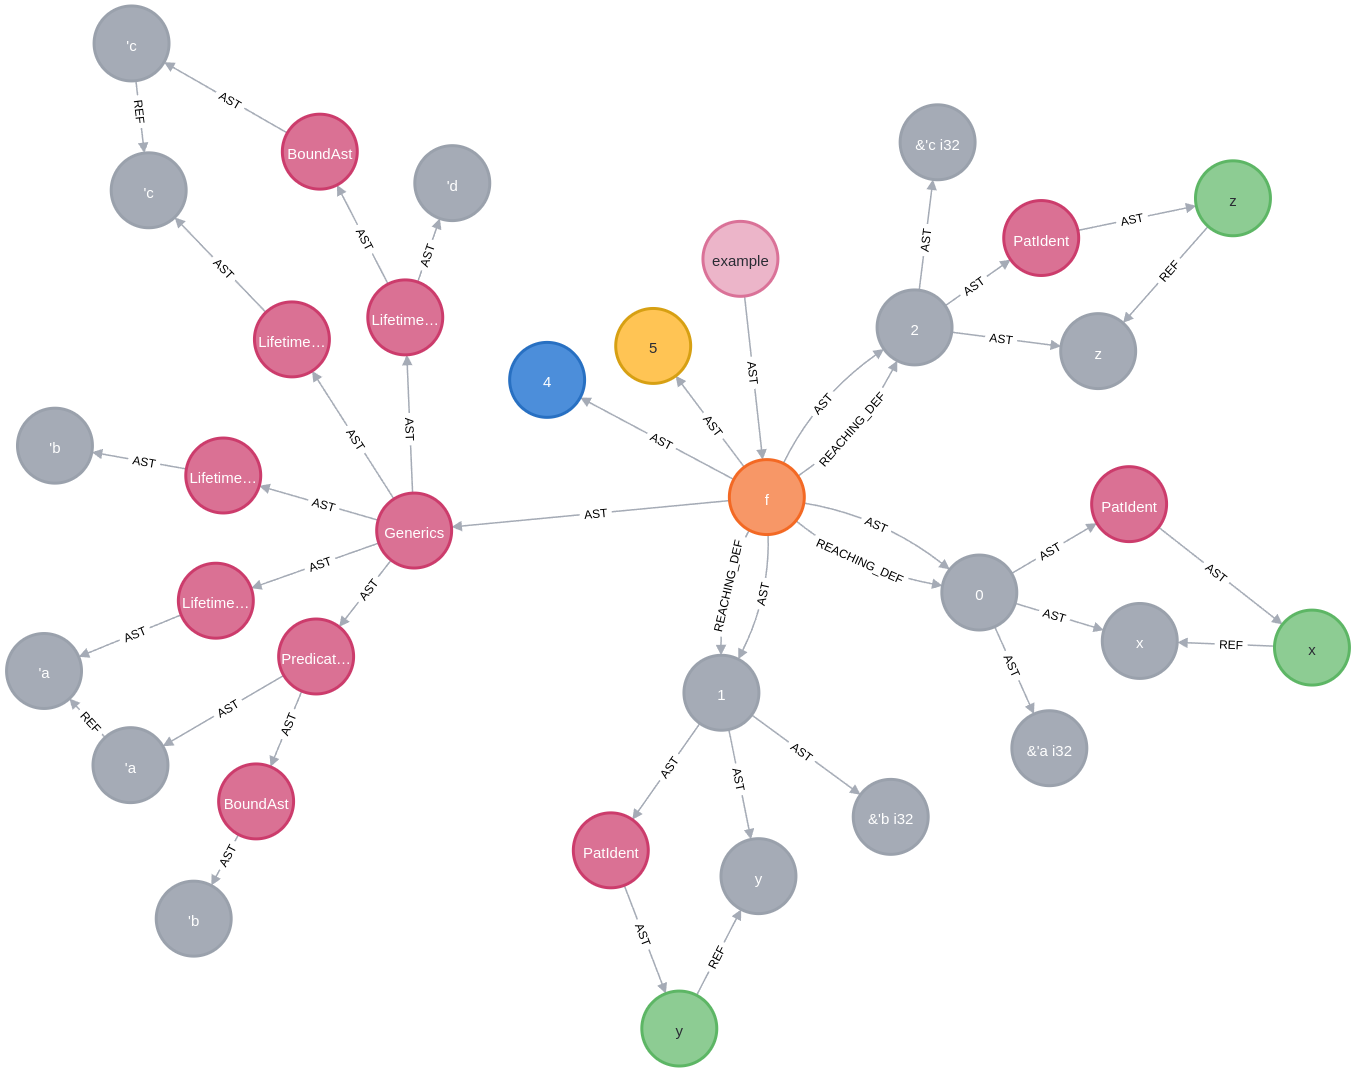
\includegraphics[width=1\columnwidth]{figures/c5/c5_lifetime_2.png}
    \centering
    \caption{Ví dụ đồ thị CPG cho đoạn mã nguồn \ref{code:c5_lifetime_2}}
    \label{img:c5_lifetime_2}
\end{figure}

% \section{Hạn chế}

\subsection{Macro}

Trong ngôn ngữ lập trình C/C++ và Rust có tính năng macro, là cách viết mã nguồn để sinh ra mã nguồn khác \cite{rustlangMacrosRust}.
Macro trong Rust bao gồm 2 loại declarative macro và procedural macro.
Declarative macro giống như macro trong C/C++, còn procedural macro giống như inline function.
Đối C/C++ có bộ tiền xử lý để xử lý macro trước khi cho vào trình biên dịch, đo đó khi mã nguồn sau khi được tiền xử lý thì đã được xử lý toàn bộ macro.
Tuy nhiên, Rust không giống C/C++, macro trong Rust không được xử lý ở trước khi sinh cây AST mà sẽ được xử lý sau khi sinh cây AST nhưng trước khi đi vào pha phân tích ngữ cảnh của trình biên dịch.
Như đã đề cập ở phần các trước, công cụ hiện tại sử dụng thư viện syn để sinh cây AST cho mã nguồn và syn không hỗ trợ xử lý macro.
Do đó tất cả các mã lệnh nằm bên trong macro sẽ không được xử lý, dẫn đến việc không thể sinh cây AST cho đoạn mã lệnh sử dụng macro.
Tất cả các đoạn lệnh nằm trong một lời gọi macro hiện tại được xem như một chuỗi ký tự.
Không chỉ vậy macro trong Rust sử dụng DSL (Domain-Specific Language) riêng, DSL này gần với ngôn ngữ Rust nhưng có sự mở rộng biến đổi để phù hợp với vai trò macro, do đó không thể sinh cây AST cho macro.

Để xử lý trường hợp trên, một bước tiền xử lý mã nguồn có thể được thêm vào để mở rộng macro như C/C++.
Công cụ có thể sử dụng đến thư viện \texttt{cargo-expand}, thư viện này có tác dụng đưa đoạn mã macro mà lập trình viên nhìn thấy thành đoạn mã mà trình biên dịch nhìn thấy.
Mã nguồn sau khi được mở rộng thì sẽ có được các thông tin bị ẩn đi như \texttt{prelude} mặc định của Rust bao gồm các hàm, các ký tự được nạp sẵn trong ngôn ngữ, các macro sẽ được mở rộng, bao gồm cả declarative và procedural macro.
Đối với declarative macro, thì macro nạp sẵn của ngôn ngữ như \texttt{println!}, \texttt{vec!} hay kể cả declarative macro do người dùng định nghĩa cũng sẽ được xử lý.
Tuy nhiên, việc mở rộng macro trước khi cho vào cây AST sẽ làm cho mã nguồn bị biến đổi so với mã nguồn gốc, đồng thời tăng kích cỡ và độ lớn của mã nguồn.
Việc thêm các thông tin ẩn mà lập trình viên không nhìn thấy có thể gây nhầm lẫn.
Điều này cũng đồng nghĩa với việc việc sinh cây AST cho mã nguồn sau khi xử lý macro sẽ phức tạp và tốn nhiều thời gian hơn.

\subsection{Module}

Cơ chế module trong Rust tương ứng với namespace trong C++, package trong Java.
Module chia nhỏ mã nguồn thành các phần nhỏ hơn, tổ chức và quản lý mã nguồn, giúp tái sử dụng mã nguồn, giúp tránh xung đột tên biến, hàm giữa các module khác nhau.
Một module trong Rust có thể là một tệp riêng biệt hoặc một phần của một tệp khác.
Các module có thể được tổ chức thành một hệ thống phân cấp, với các module con được khai báo bên trong các module cha.
% Có một số tệp được coi là tệp đặc biệt trong cấu trúc mã nguồn trong rust.
% Ví dụ như tệp mod.rs, đây là tệp module gốc của thư mục chứa nó, tất cả các module con trong thư mục đó sẽ được import thông qua module gốc mod.rs.
% Ngoài ra còn có tệp main.rs, lib.rs để đánh dấu điểm đầu vào của chương trình và xác định xem dự án là một thư viện hay một ứng dụng.
Rust còn cung cấp cơ chế workspace, cho phép quản lý nhiều dự án nhỏ trong cùng một dự án lớn, mỗi dự án là một thư mục con trong thư mục workspace.
Để kiểm soát khả năng truy cập, Rust sử dụng cơ chế visibility.
Mặc định các thành phần trong module là private, để làm cho chúng có thể truy cập được từ các module khác, ta sử dụng từ khóa \texttt{pub}.
Cơ chế path resolution dùng để định danh một thành phần cấu trúc từ module khác ta mà ta có thể import.
Path resolution có thể là đường dẫn tuyệt đối hoặc tương đối.
Ví dụ dùng từ khóa \texttt{self} để chỉ tới module hiện tại, dùng từ khóa \texttt{super} để chỉ tới module cha của module hiện tại, \texttt{crate} để chỉ tới module gốc của dự án.
Hệ thống module phức tạp của Rust làm tăng đáng kể độ khó việc xử lý quan hệ giữa các module trong cây AST và phân tích ngữ cảnh.
Việc xử lý các khái niệm như module con, module gốc, visibility, import và path resolution đòi hỏi một cơ chế phân tích tinh vi, do vậy hiện tại công cụ chưa xử lý được module.

% \subsection{Path}

% \begin{itemize}
%     \item Path có thể là Absolute Path hoặc Relative Path tùy vào bối cảnh module hiện tại, path có thể chỉ tới đối tượng trong cùng một module hoặc khác module
%     \item Path trong Rust là đường dẫn đến một đối tượng nào đó được định nghĩa trong mã nguồn như struct, trait, static, const, function
%     \item Cây AST sử dụng thư viện $syn$, $syn$ có thể lấy được path của một đối tượng nhưng không biết được đối đượng đang trỏ tới là static, const, hay function.
% Do đó đang không phân biệt được đâu là path của static, const, hay function
% \end{itemize}

% \subsection{Type Argument match Type Parameter}


\section{Ứng dụng phân tích mã nguồn có lỗ hổng bảo mật}

Tính đến năm 2023, tổng cộng có 17 thể loại bug được báo cáo về RUSTSEC Database \cite{zheng2023closer}.
Trong đó, lỗi về an toàn bộ nhớ và đa luồng chiếm tới gần hai phần ba tổng số loại lỗi.
Mặc dù Rust có các cơ chế để khắc phục những lỗi này, nhưng dường như trong những dự án thực tế phức tạp, vẫn tồn tại một số lỗi nhất định, đặc biệt khi sử dụng tính năng \texttt{unsafe} (mã không an toàn) của Rust.
Để minh họa cho việc áp dụng đồ thị CPG vào thực tế, khóa luận sẽ trình bày ứng dụng của đồ thị CPG trên 4 lỗi trong RUSTSEC Database thuộc các thể loại lỗi phổ biến nhất.

\subsection{RUSTSEC-2021-0086}

% Đoạn mã \ref{code:c5_RUSTSEC-2021-0086} minh họa một lỗ hổng bảo mật phổ biến liên quan đến việc khởi tạo bộ nhớ không an toàn trong Rust. Lỗi xảy ra khi sử dụng hàm \texttt{Vec::with_capacity} để tạo một vectơ có dung lượng dự kiến, sau đó tùy ý điều chỉnh độ dài của vectơ bằng hàm \texttt{set_len}. Tuy nhiên, hàm \texttt{set_len}, một hàm không an toàn, chỉ đơn thuần thay đổi kích thước của vectơ mà không khởi tạo giá trị cho các phần tử mới được thêm vào. Điều này dẫn đến tình trạng các phần tử này chứa giá trị rác, tiềm ẩn nhiều nguy cơ như lỗi tràn bộ nhớ, truy cập trái phép vào vùng nhớ và các vấn đề bảo mật nghiêm trọng khác.

% Để khắc phục lỗi này, Rust cung cấp macro \texttt{vec!} giúp khởi tạo vectơ một cách an toàn hơn. Khi sử dụng macro này, chúng ta có thể chỉ định rõ độ dài và giá trị ban đầu cho các phần tử của vectơ, đảm bảo rằng tất cả các phần tử đều được khởi tạo với giá trị mong muốn. Trong hình \ref{img:c5_RUSTSEC-2021-0086}, nút \texttt{BLOCK} với thuộc tính \texttt{unsafe} đánh dấu rõ ràng vùng mã không an toàn, trong khi các nút con của nó thể hiện các hoạt động cụ thể có khả năng gây ra lỗi.

Đoạn mã \ref{code:c5_RUSTSEC-2021-0086} minh họa một lỗ hổng bảo mật phổ biến liên quan đến việc khởi tạo bộ nhớ không an toàn trong Rust.
Lỗi xảy ra khi sử dụng hàm \texttt{Vec::with\_capacity} để tạo một vectơ có dung lượng được định sẵn là $N$, sau đó tùy chỉnh độ dài của vectơ bằng hàm \texttt{set\_len}.
Tuy nhiên hàm \texttt{set\_len}, một hàm được coi là \texttt{"unsafe"}, chỉ đơn thuần thay đổi kích thước của vectơ mà không khởi tạo giá trị cho các phần tử mới được thêm vào.
Điều này dẫn đến tình trạng các phần tử này chứa giá trị rác, tiềm ẩn nhiều nguy cơ như lỗi tràn bộ nhớ, truy cập trái phép vào vùng nhớ và các vấn đề bảo mật nghiêm trọng khác.
Để sửa lỗi, ta có thể sử dụng macro \texttt{vec!} để khởi tạo vectơ với độ dài và dung lượng là $N$, giá trị mặc định của mỗi phần tử là $0$.
% Trong hình \ref{img:c5_RUSTSEC-2021-0086}, nút \texttt{BLOCK} với thuộc tính \texttt{unsafe} biểu diễn việc bắt đầu một khối lệnh không an toàn.
Trong hình \ref{img:c5_RUSTSEC-2021-0086}, nút \texttt{BLOCK} với thuộc tính \texttt{unsafe} đánh dấu rõ ràng vùng mã không an toàn.
Các nút con của nút \texttt{BLOCK} này biểu diễn các mệnh đề, lời gọi hàm không an toàn.

\begin{listing}[H]
\begin{minted}[mathescape, breaklines, frame=lines, framesep=2mm, baselinestretch=1.2, fontsize=\footnotesize, linenos]{rust}
// Before fix
let mut buf: Vec<u8> = Vec::with_capacity(N);
unsafe { buf.set_len(N) };
// After fix
let mut buf: Vec<u8> = vec![0; N];
\end{minted}
\caption{Ví dụ mã nguồn cho RUSTSEC-2021-0086.}
\label{code:c5_RUSTSEC-2021-0086}
\end{listing}

\begin{figure}[H]
    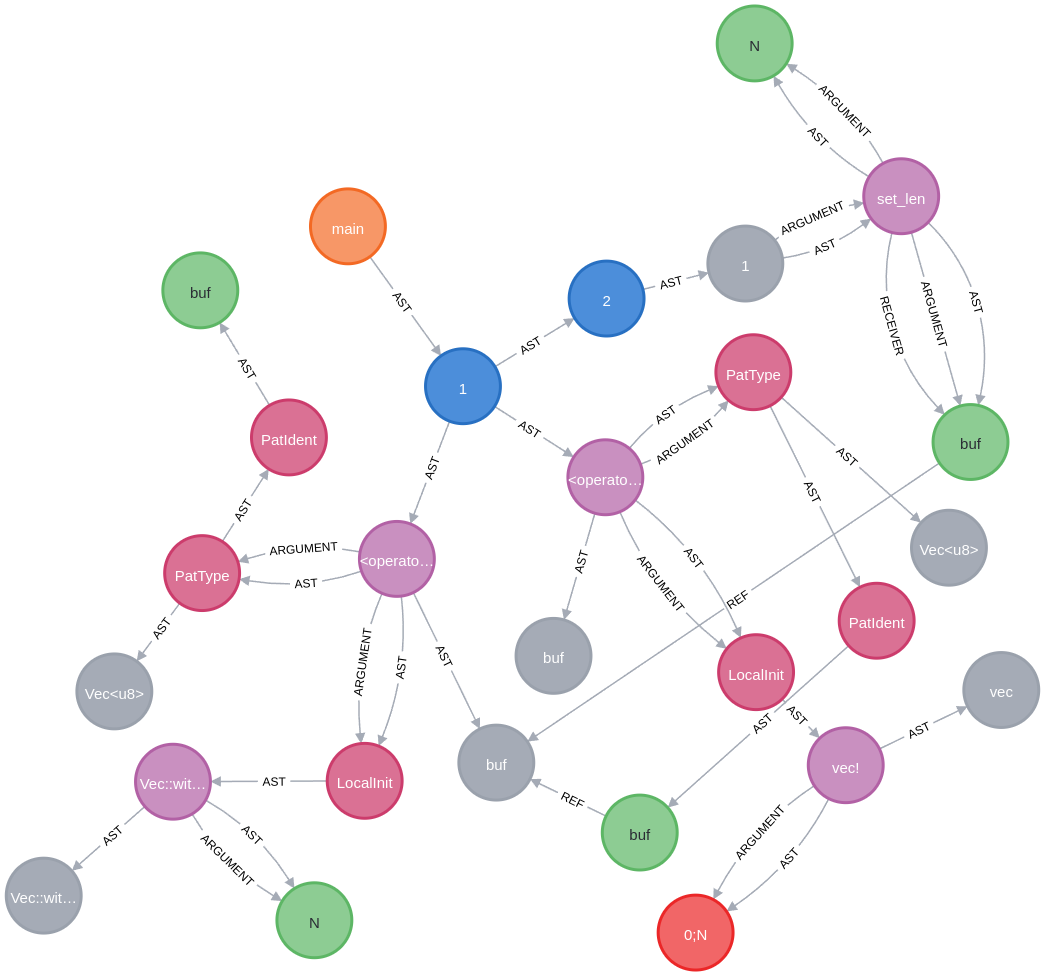
\includegraphics[width=1\columnwidth]{figures/c5/c5_RUSTSEC-2021-0086}
    \centering
    \caption{Ví dụ đồ thị CPG cho đoạn mã nguồn RUSTSEC-2021-0086 \ref{code:c5_RUSTSEC-2021-0086}.}
    \label{img:c5_RUSTSEC-2021-0086}
\end{figure}

\subsection{RUSTSEC-2022-0028}

\begin{listing}[H]
\begin{minted}[mathescape, breaklines, frame=lines, framesep=2mm, baselinestretch=1.2, fontsize=\footnotesize, linenos]{rust}
// Before fix
pub fn external<'a, T>(data: T) -> Handle<'a, Self>
where
    T: AsMut<[u8]> + Send,
{
    // ...
}
// After fix
pub fn external<'a, T>(data: T) -> Handle<'a, Self>
where
    T: AsMut<[u8]> + Send + 'static,
{
    // ...
}
\end{minted}
\caption{Ví dụ mã nguồn cho RUSTSEC-2022-0028.}
\label{code:c5_RUSTSEC-2022-0028}
\end{listing}

Đoạn mã \ref{code:c5_RUSTSEC-2022-0028} mô tả lỗi xảy ra khi sử dụng hàm \texttt{external} mà không xác định đúng ràng buộc lifetime cho kiểu tổng quát \texttt{T}.
Trong bối cảnh này, \texttt{external} là hàm được dùng để tạo ra dữ liệu giao tiếp chung giữa Rust và Javascript thông qua Web Assembly Binding \cite{ githubGitHubRustwasmwasmbindgen}.
Việc kiểu tổng quát \texttt{T} không được xác định đúng lifetime cho phép tạo ra một vùng dữ liệu có thể bị giải phóng trong khi chúng vẫn được tham chiếu bởi mã nguồn Javascript.
Để hai ngôn ngữ có thể giao tiếp được thì dữ liệu đó phải tồn tại trong suốt thời gian chạy của cả hai ngôn ngữ.
Để sửa lỗi, cần thêm ràng buộc \texttt{T: 'static} để đảm bảo rằng dữ liệu được tham chiếu sẽ không bị giải phóng trong suốt thời gian tồn tại của chương trình.
Lỗi RUSTSEC-2022-0028 là một lỗi thực sự rất khó để phát hiện tự động vì nó liên quan đến bối cảnh bài toán, ở đây là giao tiếp giữa 2 ngôn ngữ Rust và Javascript thông qua Web Assembly Binding.
Hình \ref{img:c5_RUSTSEC-2022-0028} cũng thể chưa trình bày một cách rõ ràng lỗi có thể xảy ra khi sử dụng hàm \texttt{external} và kiểu tổng quát \texttt{T}, do cần đến bối cảnh bài toán.
Nếu sử dụng đồ thị CPG kết hợp với các mẫu khai phá để tự động phân tích thì chưa thể phát hiện ra lỗ hổng.
Do cần kiến thức về bối cảnh bài toán nên sự can thiệp của con người là cần thiết trong trường hợp này.
Các câu truy vấn đồ thị CPG kết hợp với kiến thức miền của các chuyên gia có thể được xây dựng thủ công mới có thể phát hiện ra lỗi.

% \begin{listing}[H]
% \begin{minted}[mathescape, breaklines, frame=lines, framesep=2mm, baselinestretch=1.2, fontsize=\footnotesize, linenos]{rust}
% // Before fix
% pub fn external<'a, C, T>(cx: &mut C, data: T) -> Handle<'a, Self>
% where
%     C: Context<'a>,
%     T: AsMut<[u8]> + Send,
% {
%     // ...
% }

% // After fix
% pub fn external<'a, C, T>(cx: &mut C, data: T) -> Handle<'a, Self>
% where
%     C: Context<'a>,
%     T: AsMut<[u8]> + Send + 'static,
% {
%     // ...
% }
% \end{minted}
% \caption{Ví dụ mã nguồn cho RUSTSEC-2022-0028}
% \label{code:c5_RUSTSEC-2022-0028}
% \end{listing}


\begin{figure}[H]
    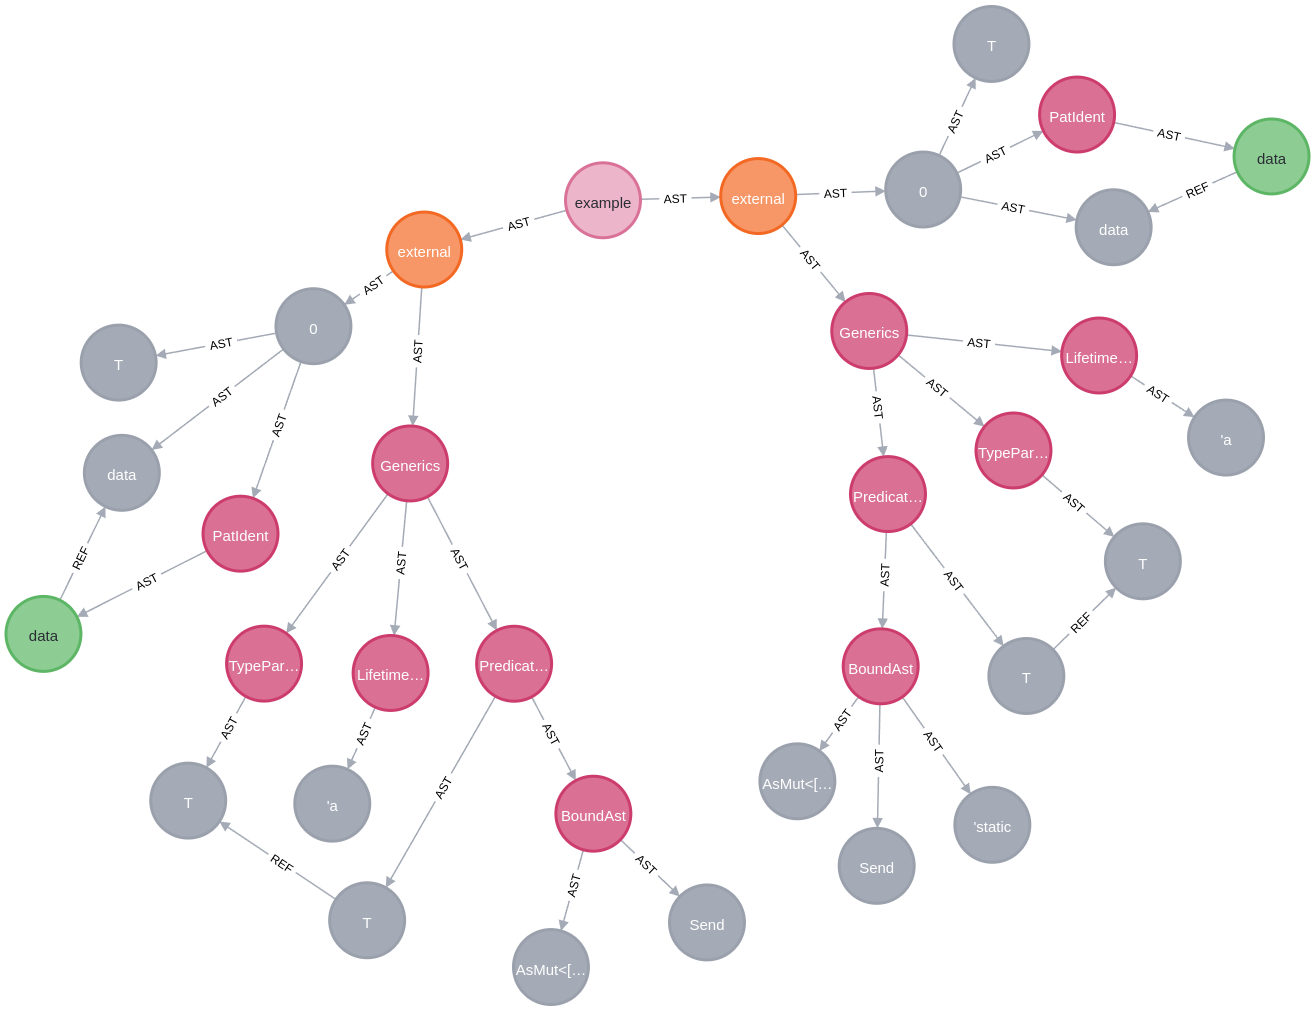
\includegraphics[width=1\columnwidth]{figures/c5/c5_RUSTSEC-2022-0028.png}
    \centering
    \caption{Ví dụ đồ thị CPG cho đoạn mã nguồn RUSTSEC-2022-0028 \ref{code:c5_RUSTSEC-2022-0028}.}
    \label{img:c5_RUSTSEC-2022-0028}
\end{figure}


\subsection{RUSTSEC-2020-0044}


\begin{listing}[H]
\begin{minted}[mathescape, breaklines, frame=lines, framesep=2mm, baselinestretch=1.2, fontsize=\footnotesize, linenos]{rust}
// Before fix
unsafe impl<P> Send for Atom<P> where P: IntoRawPtr + FromRawPtr {}
unsafe impl<P> Sync for Atom<P> where P: IntoRawPtr + FromRawPtr {}

// After fix
unsafe impl<P> Send for Atom<P> where P: IntoRawPtr + FromRawPtr + Send {}
unsafe impl<P> Sync for Atom<P> where P: IntoRawPtr + FromRawPtr + Sync {}
\end{minted}
\caption{Ví dụ mã nguồn cho RUSTSEC-2020-0044.}
\label{code:c5_RUSTSEC-2020-0044}
\end{listing}

Đoạn mã \ref{code:c5_RUSTSEC-2020-0044} mô tả lỗi liên quan đến việc không triển khai thuộc tính \texttt{Send} và \texttt{Sync} cho kiểu dữ liệu con bên trong kiểu \texttt{Atom}.
Trong bối cảnh này, \texttt{Atom} đóng vai trò như một hộp chứa cho kiểu dữ liệu \texttt{P} bên trong, giúp quản lý việc sử dụng bộ nhớ an toàn hơn.
Tuy nhiên chỉ mình \texttt{Atom} được cài đặt thuộc tính \texttt{Send} và \texttt{Sync}, không đảm bảo rằng kiểu dữ liệu con \texttt{P} cũng phải cài đặt thuộc tính \texttt{Send} và \texttt{Sync}.
Điều này có nghĩa việc truy cập đến \texttt{Atom} có thể an toàn nhưng khi truy cập vào dữ liệu kiểu \texttt{P} bên trong thì không an toàn, có thể dẫn đến các vấn đề như sử dụng bộ nhớ sau khi đã giải phóng hoặc tương tranh dữ liệu cho kiểu dữ liệu \texttt{P} bên trong.
Để sửa lỗi này, cần đảm bảo rằng kiểu \texttt{P} cũng phải được đánh dấu thuộc tính \texttt{Send} và \texttt{Sync}.

\begin{figure}[H]
    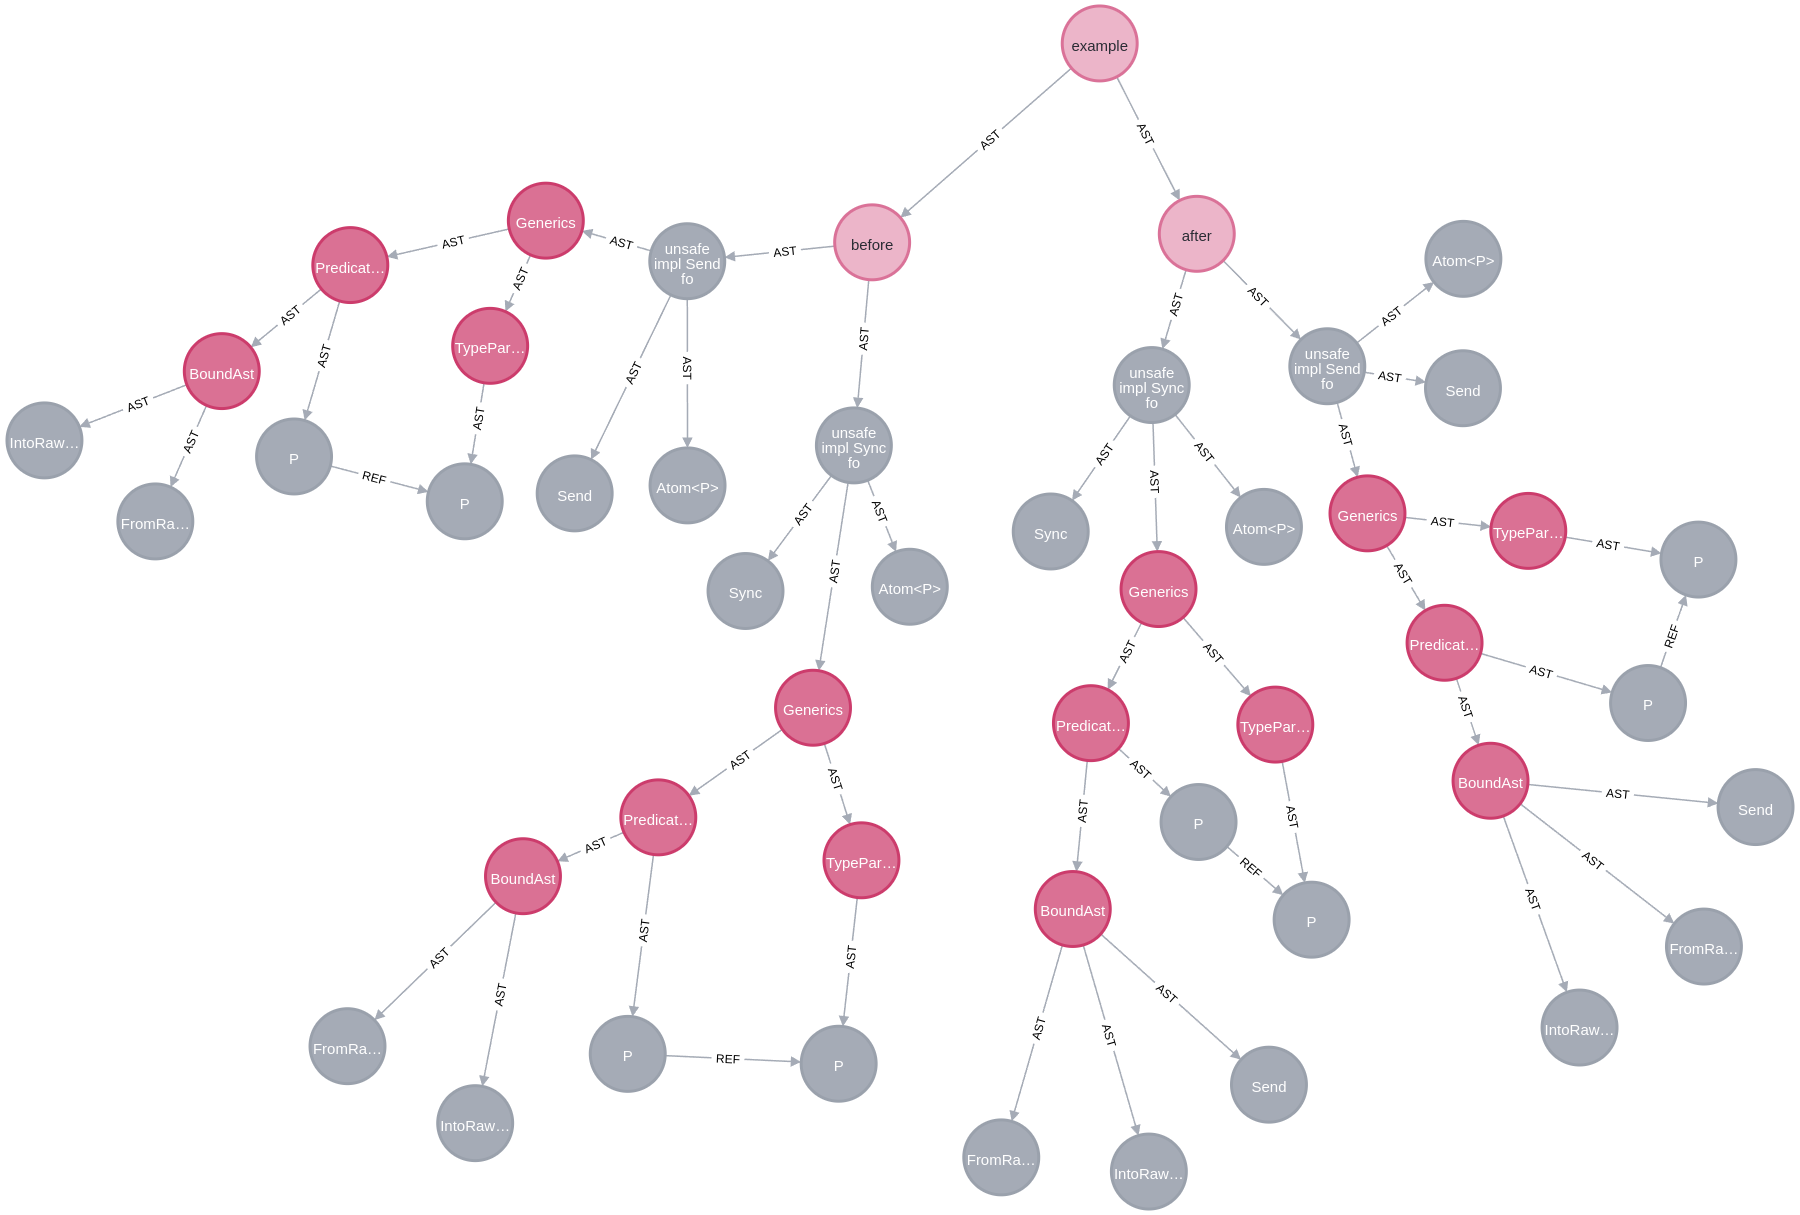
\includegraphics[width=1\columnwidth]{figures/c5/c5_RUSTSEC-2020-0044.png}
    \centering
    \caption{Ví dụ đồ thị CPG cho đoạn mã nguồn RUSTSEC-2020-0044 \ref{code:c5_RUSTSEC-2020-0044}.}
    \label{img:c5_RUSTSEC-2020-0044}
\end{figure}

Lỗi RUSTSEC-2020-0044 là một lỗi xảy ra thường xuyên khi lập trình đa luồng trong Rust.
Kiểu cha muốn đảm bảo an toàn về đa luồng thì kiểu con cũng phải đảm bảo an toàn về đa luồng.
Trong bối cảnh của Rust, điều này có nghĩa là nếu kiểu cha muốn được gửi qua các luồng một cách an toàn bằng thuộc tính \texttt{Send} và \texttt{Sync} thì kiểu con cũng phải có khả năng này.
Khi được biểu diễn trực quan trên hình \ref{code:c5_RUSTSEC-2020-0044}, hoàn toàn ta có thể thấy một mẫu duyệt đồ thị để phát hiện lỗi này.
Một mẫu khai phá đồ thị phổ biến có thể được xây dựng và sử dụng cho nhiều đoạn mã khác nhau.
Các truy vấn hoặc phân tích dựa trên mẫu này có thể được áp dụng trên đồ thị CPG để phát hiện các lỗi tương tự.

\subsection{RUSTSEC-2021-0130}

\begin{listing}[H]
\begin{minted}[mathescape, breaklines, frame=lines, framesep=2mm, baselinestretch=1.2, fontsize=\footnotesize, linenos]{rust}
// Before fix
pub fn iter<'a>(&'_ self) -> Iter<'a, K, V> {
    Iter { ptr: unsafe { (*self.head).next }, }
}
// After fix
pub fn iter(&self) -> Iter<'_, K, V> {
    Iter { ptr: unsafe { (*self.head).next }, }
}
\end{minted}
\caption{Ví dụ mã nguồn cho RUSTSEC-2021-0130.}
\label{code:c5_RUSTSEC-2021-0130}
\end{listing}


Đoạn mã \ref{code:c5_RUSTSEC-2021-0130} mô tả về một lỗi sử dụng bộ nhớ sau khi đã giải phóng.
Trong bối cảnh này, \texttt{Iter} là một \texttt{struct} được sử dụng để duyệt qua các phần tử trong một danh sách liên kết.
Tuy nhiên, khi \texttt{Iter} được trả về từ hàm \texttt{iter} thì nó sẽ trỏ tới \texttt{self.head} mà \texttt{self.head} có thể bị giải phóng trước khi \texttt{Iter} được sử dụng, dẫn đến việc sử dụng bộ nhớ sau khi đã giải phóng.
Nguyên nhân là do quan hệ lifetime giữa biến \texttt{self} và giá trị trả về kiểu \texttt{Iter} không đồng bộ.
Biến \texttt{self} được chỉ định lifetime là \texttt{'\_}, tức là để trình biên dịch tự động gán một giá trị lifetime mặc định, trong khi đó kiểu trả về \texttt{Iter} được chỉ định lifetime là \texttt{'a}.
Trong trường hợp này \texttt{'\_} và \texttt{'a} không có liên hệ với nhau do đó lifetime của \texttt{Iter} có thể lớn hơn lifetime của \texttt{self}, dẫn đến việc truy cập đến \texttt{self.head} sau khi \texttt{self} đã bị giải phóng.
Để sửa lỗi, cần sử dụng chung một lifetime cho \texttt{self} và \texttt{Iter} thông qua việc sử dụng 3 quy tắc lược bỏ lifetime \cite{rustlangLifetimeElision}.
Nếu không chỉ định lifetime một cách tường minh, ba quy tắc lược bỏ lifetime sẽ được trình biên dịch sử dụng để tự động xác định lifetime của các biến dựa trên cấu trúc của hàm, bao gồm:

\begin{enumerate}
    \item Mỗi tham số kiểu tham chiếu của hàm mặc định có một lifetime riêng.
    \item Khi hàm có một tham số kiểu tham chiếu duy nhất, và kiểu trả về cũng là kiểu tham chiếu thì lifetime của kiểu trả về sẽ là lifetime của tham số tham số kiểu tham chiếu duy nhất đó.
    \item Nếu hàm có nhiều tham số kiểu tham chiếu nhưng có một tham số là \texttt{self} (\texttt{self} tương đương với \texttt{this} trong C++ và Java), thì lifetime của \texttt{self} sẽ được gán cho kiểu tham số trả về.
\end{enumerate}

Trong trường hợp này, ta sửa lỗi bằng cách không chỉ định lifetime cho \texttt{self} mà để trình biên dịch tự xác định, lifetime của \texttt{Iter} sẽ để là \texttt{'\_}.
Ký hiệu \texttt{'\_} tức là tự động suy diễn và áp dụng quy tắc số 3 thì lifetime của \texttt{Iter} sẽ được gán bằng lifetime của \texttt{self}.
Từ đó lifetime của \texttt{Iter} sẽ không lớn hơn lifetime của \texttt{self} và việc truy cập đến \texttt{self.head} sau khi \texttt{self} đã bị giải phóng sẽ không xảy ra.

\begin{figure}[H]
    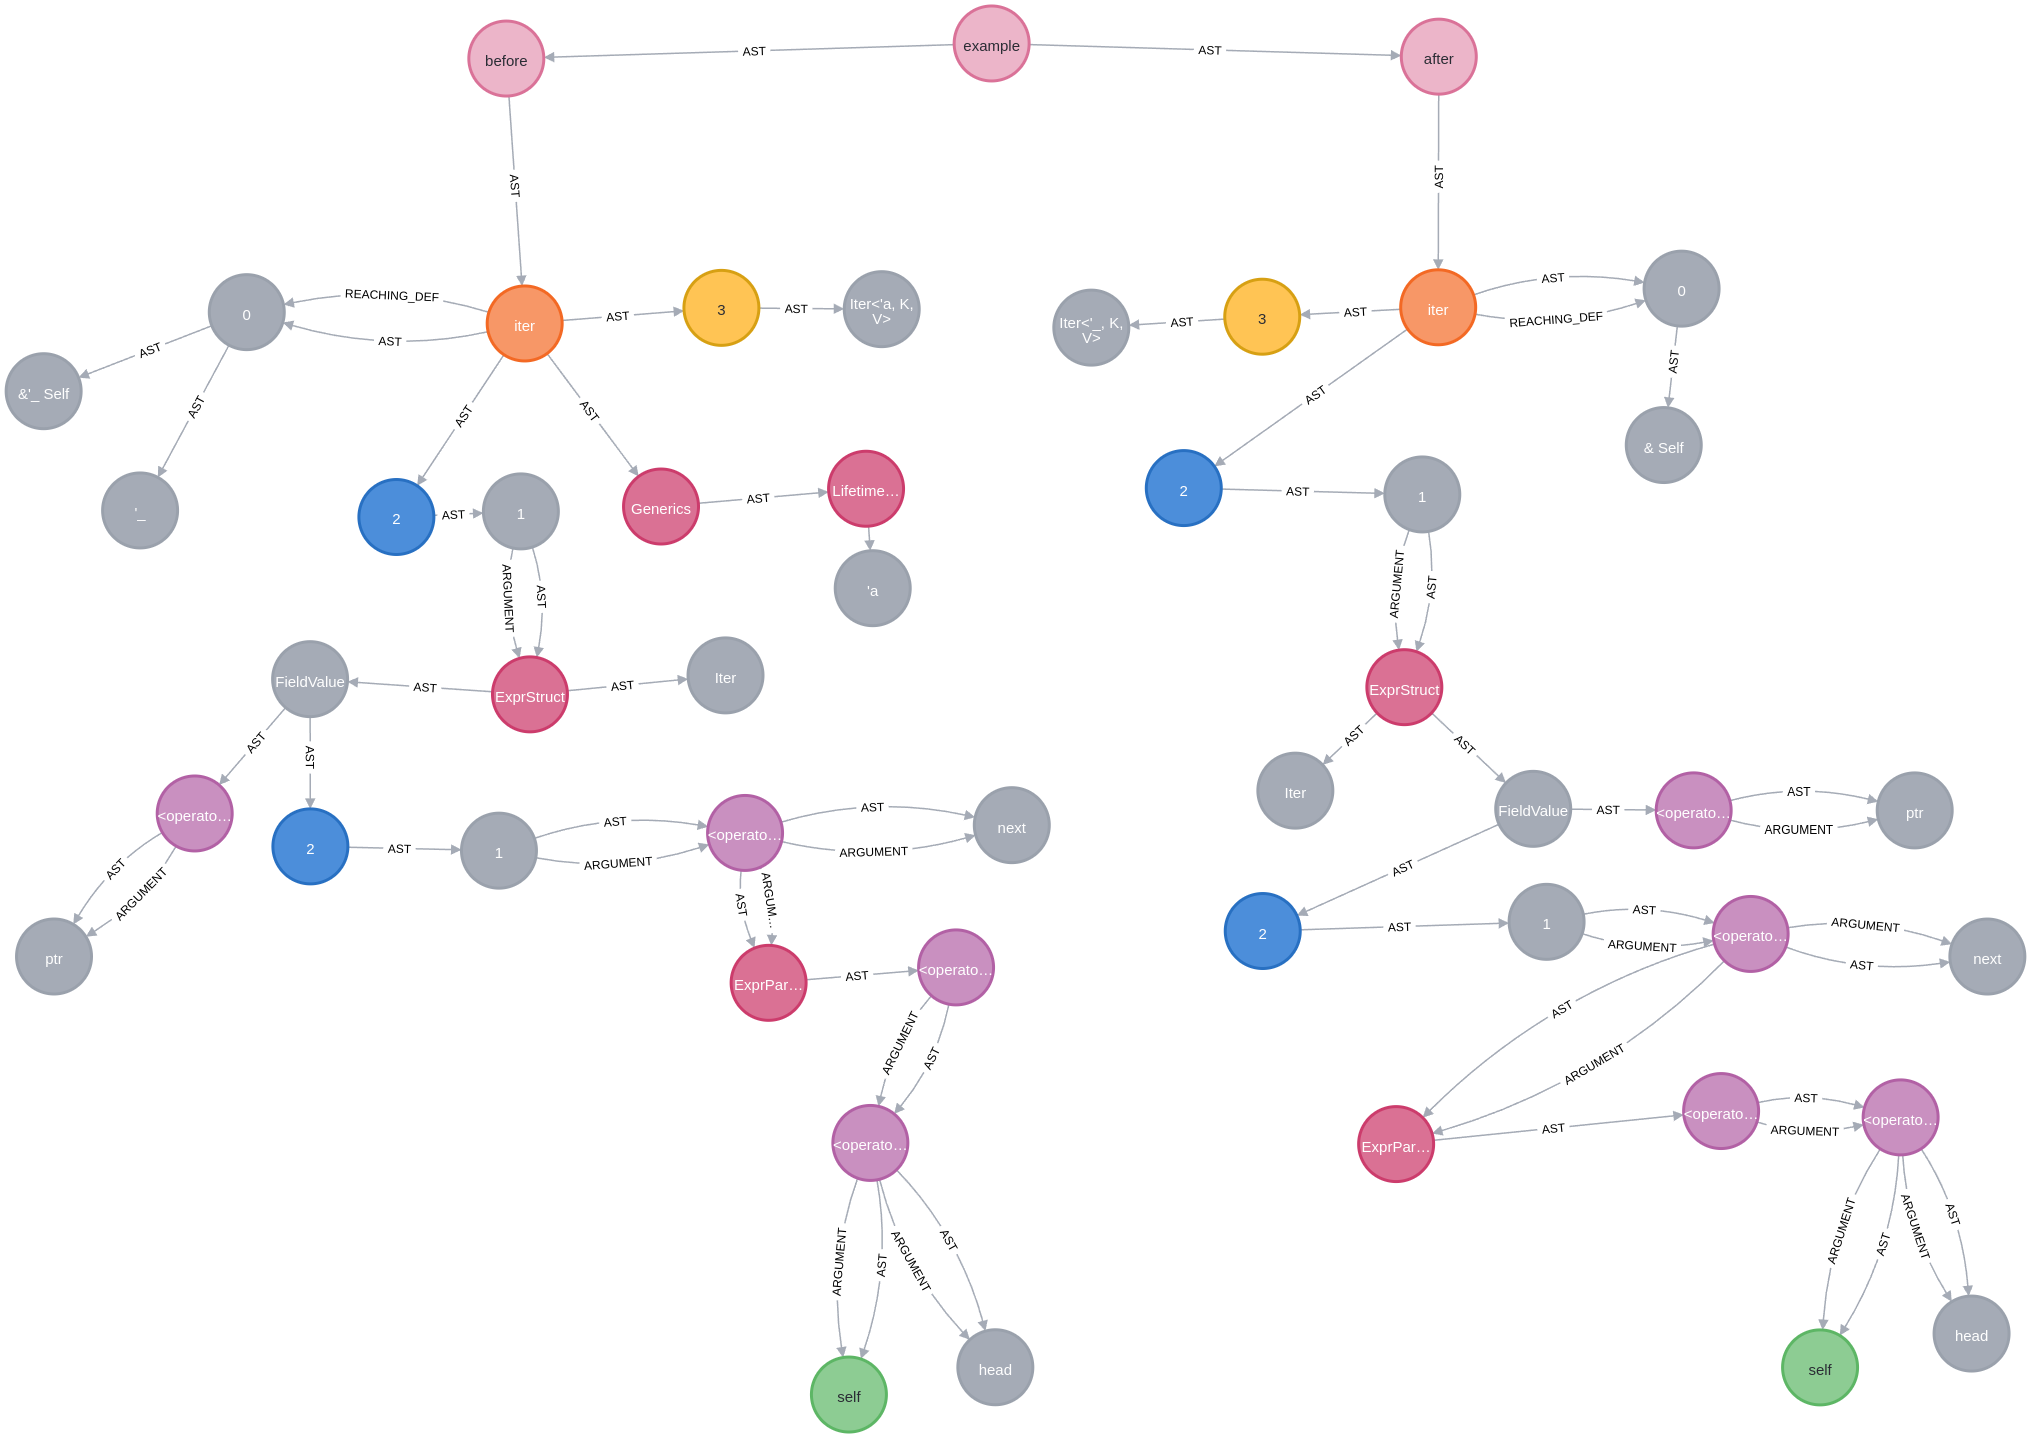
\includegraphics[width=1\columnwidth]{figures/c5/c5_RUSTSEC-2021-0130.png}
    \centering
    \caption{Ví dụ đồ thị CPG cho đoạn mã nguồn RUSTSEC-2021-0130 \ref{code:c5_RUSTSEC-2021-0130}.}
    \label{img:c5_RUSTSEC-2021-0130}
\end{figure}

Đánh dấu lifetime một cách tường minh cần được thực hiện cẩn thận để tránh được các lỗi liên quan đến bộ nhớ.
Việc đánh dấu lifetime không chính xác có thể đánh lừa trình biên dịch và dẫn đến việc sử dụng bộ nhớ sau khi đã giải phóng.
Lifetime của kiểu trả về phải đảm bảo không lớn hơn lifetime của tham số truyền vào nếu kiểu trả về có truy cập đến bộ nhớ của tham số truyền vào.
Có thể áp dụng ba quy tắc lược bỏ lifetime để suy diễn việc xác định lifetime giữa tham số và tham số, giữa tham số và kiểu trả về.
Kết hợp với đồ thị CPG \ref{img:c5_RUSTSEC-2021-0130}, các luật có thể được đề ra để phát hiện sự không đồng bộ về lifetime giữa các biến dựa vào các nút \texttt{LIFETIME},
\texttt{LIFETIME PARAMETER} và các cạnh thể hiện mối quan hệ giữa chúng như \texttt{OUT LIVE}, \texttt{REF}.

\section{Thực nghiệm học máy trên đồ thị CPG}

% Mục tiêu thực nghiệm là Bài toán phân loại
% Dữ liệu
% Độ đo đánh giá
% Baseline
% Kết quả thực nghiệm

Để chứng minh tiềm năng của đồ thị CPG dành cho ngôn ngữ Rust, khóa luận xây dựng một thực nghiệm sử dụng học máy để phát hiện lỗ hổng bảo mật mã nguồn Rust dựa trên đồ thị CPG.
Bài toán đặt ra là phân loại tệp mã nguồn Rust có lỗ hổng bảo mật và không có lỗ hổng bảo mật.
Thực nghiệm sẽ tiến hành so sánh độ hiệu quả giữa mô hình học máy sử dụng đồ thị CPG và mô hình học máy học sử dụng mã nguồn Rust truyền thống.
Mô hình học máy chỉ sử dụng dữ liệu mã nguồn Rust, tạm gọi là Baseline, sẽ sử dụng kĩ thuật Word2Vec để biểu diễn mã nguồn và Logistic Regression để phân loại.
Đối với bài toán học máy để phát hiện lỗ hổng bảo mật trên đồ thị CPG, trước đây đã có mô hình Devign, một mô hình kinh điển cho lớp bài toán này \cite{zhou2019devign}.
Devign đã được sử dụng cho ngôn ngữ C/C++ và cũng sử dụng Joern, do đó Devign hoàn toàn có thể sử dụng tương tự cho CPG của ngôn ngữ Rust trong khóa luận này.

Bộ dữ liệu được sử dụng bao gồm 260 tệp mã nguồn Rust, trong đó 130 tệp có lỗ hổng bảo mật và 130 tệp không có lỗ hổng bảo mật.
Đối với 130 tệp có lỗ hổng bảo mật, dữ liệu được trích xuất từ bài báo khoa học "A Closer Look at the Security Risks in the Rust Ecosystem" \cite{zheng2023closer}.
Còn 130 tệp không có lỗ bảo mật được thu thập từ 100 dự án mã nguồn mở của Rust nhiều sao nhất trên Github \cite{githubGithubRankingTop100RustmdMaster} và xác nhận thủ công.
Tập dữ liệu được chia thành 3 phần, 80\% dữ liệu được sử dụng cho quá trình huấn luyện, 10\% dữ liệu được sử dụng cho kiểm chứng, 10\% dữ liệu được sử dụng cho kiểm thử.

Với bài toán phân loại, thang đo đánh giá hiệu suất của mô hình sẽ bao gồm các chỉ số Accuracy, Precision, Recall và F1-score.
% ROC AUC, Precision-Recall AUC, MCC, Error Rate
Để đánh giá hiệu suất, mỗi mô hình được chạy 10 lần đối với tập dữ liệu như trên.
Kết quả của các chỉ số là giá trị trung bình của 10 lần chạy.
Kết quả thực nghiệm được thể hiện trong bảng \ref{table:c5_ml}.

\begin{table}[H]
    \centering
    \caption{Bảng so sánh mô hình Baseline và mô hình Devign}
    \label{table:c5_ml}
    \begin{tabular}{l @{\hskip 3cm} c @{\hskip 3cm} c}
        \hline
         & Baseline & \textbf{Devign (Rust)} \\
        \hline
        Accuracy & 0.73 & \textbf{0.77} \\
        Precision & 0.73 & \textbf{0.77} \\
        Recall & 0.70 & \textbf{0.99} \\
        F1-score & 0.72 & \textbf{0.87} \\
        % ROC AUC & 0.81 & \textbf{0.47} \\
        % Precision-Recall AUC & 0.74 & \textbf{0.78} \\
        % MCC & 0.46 & \textbf{0.01} \\
        % Error Rate & 0.27 & \textbf{0.23} \\
        \hline
    \end{tabular}
\end{table}

Trong bảng \ref{table:c5_ml}, mô hình Devign đã cho kết quả tốt hơn so với mô hình Baseline với hầu hết các chỉ số.
Ta thấy được Accuracy hơn 0.04, Precision hơn 0.04, Recall hơn 0.29, F1-Score hơn 0.15.
% , Precision-Recall AUC hơn 0.04 và Error Rate thấp hơn 0.04.
% Tuy nhiên, ROC AUC và MCC của mô hình Devign lại thấp hơn so với mô hình Baseline.
Điều này chứng tỏ mô hình Devign có tiềm năng áp dụng cho bài toán học máy phát hiện lỗ hổng bảo mật trên trên đồ thị CPG cho Rust.
Mã nguồn của thực nghiệm được lưu trữ tại địa chỉ \href{https://github.com/congnghiahieu/devign}{devign}.

Độ chính xác của mô hình Devign mới chỉ đạt được ở mức 0.77 bởi một vài nguyên do.
Thứ nhất là kích cỡ của bộ dữ liệu cho ngôn ngữ Rust, hiện tại các mã nguồn có lỗi được xác nhận đều lấy từ RUSTSEC Database.
Rust là ngôn ngữ mới phát triển gần đây, hệ sinh thái chưa lớn mạnh nên số lượng mã nguồn có lỗi được báo cáo không nhiều.
Thứ hai là đồ thị CPG của Rust vẫn chưa đầy đủ hoàn toàn.
Tồn tại các tính năng của Rust như marco, module chưa thể phân tích ra cây AST hay lấy các thông tin liên hệ giữa các nút.
% Các lớp thông tin về CFG, PDG vẫn chưa được hoàn thiện, hay các lớp thông tin khác có giá trị khai thác được sinh ra từ Joern cũng chưa được cung cấp.
Thứ ba là hạn chế cài đặt của mô hình Devign.
Phiên bản cài đặt của Devign là mô phỏng lại từ bài báo khoa học gốc.
Hiện tại Devign chỉ có thể sử dụng lớp thông tin về AST và CFG mà không có PDG, do vậy không thể khai thác được hết toàn bộ thông tin từ đồ thị CPG.
% chưa kể các lớp thông tin khác của Joern CPG.
Nếu có thể khắc phục được các hạn chế kể trên, mô hình Devign có thể đạt được kết quả tốt hơn nữa.
Dù tồn tại những hạn chế, kết quả thực nghiệm vẫn cho thấy tiềm năng khai thác to lớn của đồ thị CPG cho ngôn ngữ Rust.
Đồ thị CPG có thể được sử dụng cho các lớp bài toán cần đến phân tích mã nguồn như phát hiện lỗ hổng bảo mật, phân loại mã nguồn hay các ứng dụng khác trong tương lai.


